% Generated by pipeline/paper/scripts/make_result_figures.py. Do not edit by hand.
% Derived indicative ratio, stock 38.2 over the E2 driver sum.
% Shared figure style. Input once; a second input is a no-op.
\ifdefined\actsplotsready
\else
  \def\actsplotsready{1}
  \colorlet{actsteal}{teal!72!black}
  \colorlet{actstealfaint}{teal!16}
  \colorlet{actsorange}{orange!88!black}
  \colorlet{actsink}{black!80}
  \colorlet{actsghost}{black!45}
  \colorlet{actsfail}{red!62!black}
  \colorlet{actsrule}{black!50}
  \usetikzlibrary{intersections}
  \usepgfplotslibrary{fillbetween,groupplots}
  \pgfplotsset{
    acts/.style={
      font=\scriptsize\sffamily,
      tick label style={font=\scriptsize\sffamily},
      label style={font=\scriptsize\sffamily},
      legend style={
        font=\scriptsize\sffamily,
        draw=none,
        fill=none,
        cells={anchor=west},
        inner sep=1pt,
        column sep=6pt
      },
      legend cell align=left,
      scale only axis,
      clip=false,
      axis line style={actsrule},
      tick style={actsrule},
      tick align=outside,
      axis lines=left,
      xmajorgrids=true,
      major grid style={black!7},
      ymajorgrids=false,
      every node/.append style={font=\scriptsize\sffamily, inner sep=1.5pt},
      every axis plot/.append style={line join=round, line cap=round},
    },
  }
  \tikzset{
    actlab/.style={
      font=\scriptsize\sffamily,
      fill=white,
      fill opacity=0.92,
      text opacity=1,
      inner sep=1.35pt,
      outer sep=0.5pt,
    },
  }
\fi

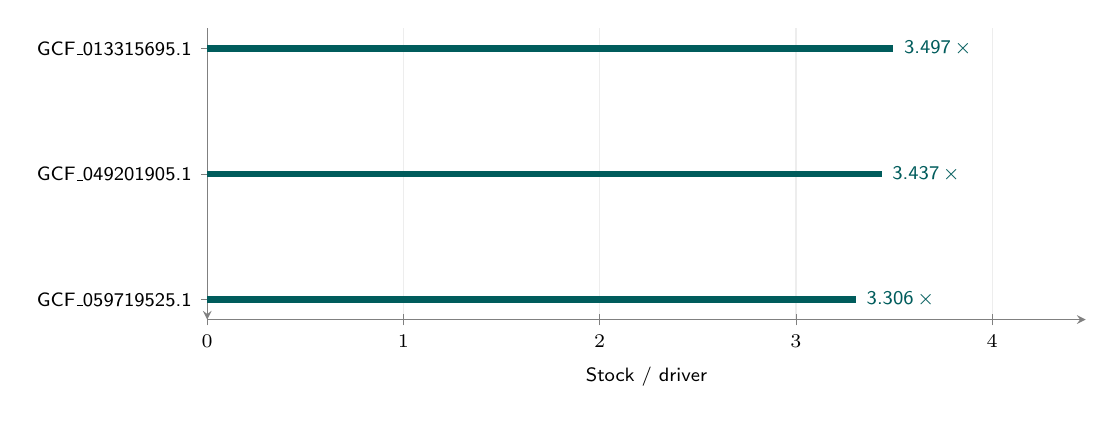
\begin{tikzpicture}
\begin{axis}[
  acts,
  width=0.92\columnwidth,
  height=3.70cm,
  xmin=0, xmax=4.47623,
  xtick={0,1,2,3,4},
  xlabel={Stock / driver},
  symbolic y coords={r0,r1,r2},
  ytick={r0,r1,r2},
  y dir=reverse,
  yticklabels={{GCF\_013315695.1},{GCF\_049201905.1},{GCF\_059719525.1}},
  enlarge y limits=0.08,
]
\addplot[draw=none, forget plot] coordinates {(0,r0) (0,r1) (0,r2)};
% source: derived from exact_replay/e1scale.json
\draw[actsteal, line width=2.4pt, line cap=butt] (axis cs:0,r0) -- (axis cs:3.4970554,r0);
\node[actlab, anchor=west, text=actsteal, xshift=2pt] at (axis cs:3.4970554,r0) {3.497\,$\times$};
\draw[actsteal, line width=2.4pt, line cap=butt] (axis cs:0,r1) -- (axis cs:3.4373635,r1);
\node[actlab, anchor=west, text=actsteal, xshift=2pt] at (axis cs:3.4373635,r1) {3.437\,$\times$};
\draw[actsteal, line width=2.4pt, line cap=butt] (axis cs:0,r2) -- (axis cs:3.3064029,r2);
\node[actlab, anchor=west, text=actsteal, xshift=2pt] at (axis cs:3.3064029,r2) {3.306\,$\times$};
\end{axis}
\end{tikzpicture}
